\subsubsubsection{Case IV: Scene-by-Scene Historical Video Understanding}
\label{case_video_history}

\begin{center}
\CaseInputTitle{Input Video}\\[0.4em]
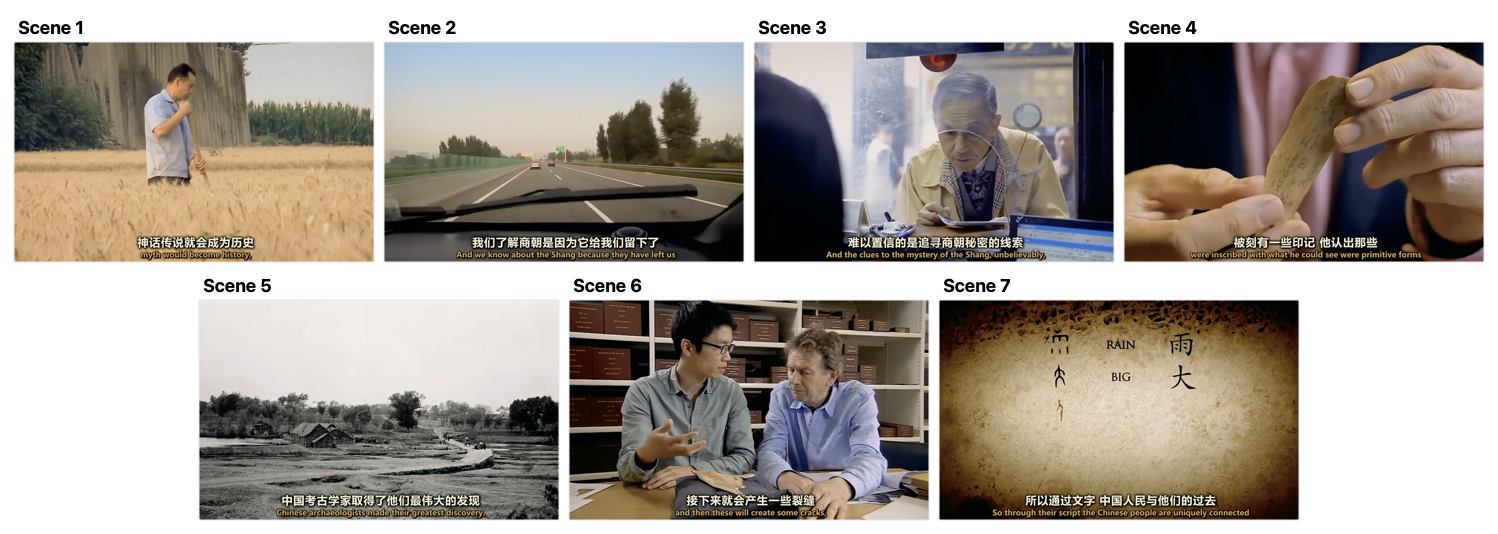
\includegraphics[width=0.88\linewidth]{arXiv/cases/figs/history_video_preview.png}
\end{center}

\begin{caseprompt}
Describe the content of the video by scene and present it in English.
\end{caseprompt}

\begin{caseresponse}
\textbf{Scene 1: Opening Rural Landscape and Mythical History.}
The video begins with a yellow flag waving against a clear sky, framed by lush green trees. The scene transitions to a vast golden wheat field where a farmer harvests crops with a sickle. Children ride bicycles along a rural road, passing by motorbikes. Subtitles state, ``If this was the capital of the Xia, for the Chinese, myth would become history, for they would have found the root of the Chinese state.''

\textbf{Scene 2: Highway Journey and Historical Transition.}
A man drives on a highway, with the rearview mirror reflecting his face. Subtitles mention ``around 1200 BC'' and the search for China's earliest historical rulers, specifically the Shang Dynasty, noted for leaving the ``first Chinese writing.'' The camera shows a roadside statue of a laughing Buddha and highway traffic.

\textbf{Scene 3: Traditional Street and Chinese Medicine Store.}
The scene shifts to a bustling traditional street with pedestrians, a child blowing bubbles, and ornate architectural details. It transitions inside an old Chinese medicine store, where staff prepare herbal packages, and a foreign man navigates the crowded pharmacy. Subtitles highlight the Shang Dynasty's discovery as ``one of the most exciting stories in world archaeology'' and emphasize traditional Chinese medicine's ancient roots.

\textbf{Scene 4: Wang Yirong's Discovery of Oracle Bones.}
Inside the pharmacy, the foreign man recounts the story of Wang Yirong in 1899, a Beijing Hanlin Academy chancellor who, while ill with malaria, purchased medicine containing ``dragon bones,'' namely animal bones. Upon opening the package, he discovered inscriptions resembling ancient bronze writings, leading to the tracing of these bones to Anyang, Henan. Close-ups show him examining the inscribed bones.

\textbf{Scene 5: Anyang Archaeological Excavation.}
Black-and-white historical photos depict the Anyang excavation site, showing massive tombs of late Shang kings with human sacrifices and rows of skulls. Subtitles note that the 1928 excavation uncovered nearly 30,000 oracle bones documenting divination activities of nine Shang kings. The sequence includes images of archaeologists at work and close-ups of inscribed bones.

\textbf{Scene 6: Expert Discussion on Oracle Bone Divination.}
Two experts discuss the oracle bone divination process. One explains how Shang kings burned cracks in turtle shells or ox bones to communicate with ancestors, interpreting crack patterns to determine auspiciousness. They compare oracle bone characters with modern Chinese script, such as the character for ``rain,'' illustrating its evolution from pictographs to modern form.

\textbf{Scene 7: Evolution of Chinese Script Animation.}
An animated sequence illustrates the transformation from prehistoric oracle bone pictographs to modern Chinese script, showing thousands of characters linking the present to the past. Subtitles emphasize how Chinese people are uniquely connected to their history and thinking through their script, surpassing other cultures globally.
\end{caseresponse}

\captionof{figure}{\textbf{Video case for long-form scene-level understanding.} Keye-VL-2.0 summarizes a historical documentary clip by segmenting the video into coherent scenes, tracking transitions from rural landscapes and travel shots to traditional medicine, oracle-bone discovery, Anyang excavation, expert discussion, and the evolution of Chinese script.}
\label{fig:history_video_case}

\clearpage

\subsubsubsection{Case V: Daily Vlog and Equestrian Lesson Understanding}
\label{case_video_ks_daily_vlog}

\begin{center}
\centering
\CaseInputTitle{Input Video}\\[0.4em]
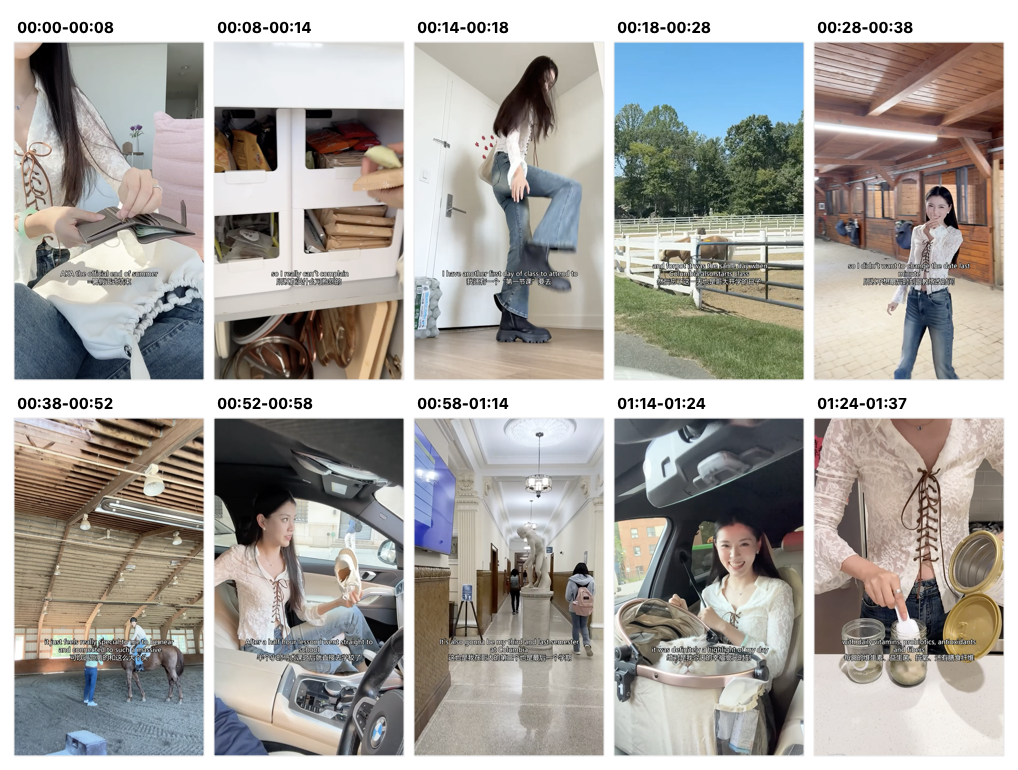
\includegraphics[width=0.66\linewidth]{arXiv/cases/figs/ks_video_preview.png}
\end{center}

\begin{caseprompt}
Describe the content of the video by scene and present it in English.
\end{caseprompt}

\begin{caseresponse}
The model segments a daily vlog into ten timestamped scenes, preserving the user's school preparation, equestrian lesson, campus classes, family interaction, and evening routine. The response below is presented as a compact timeline.

\renewcommand{\arraystretch}{1.08}
\begin{tabular}{p{0.18\linewidth}p{0.77\linewidth}}
\toprule
\textbf{Time} & \textbf{Scene summary} \\
\midrule
00:00--00:08 & \textbf{Living room preparation for school.} In a bright living room at 11:39 AM, the woman shows a white drawstring bag and its contents, including a wallet, tablet, and water bottle. On-screen text introduces the first day of class at Columbia and the end of summer break. \\
00:08--00:14 & \textbf{Kitchen snack packing.} She opens organized kitchen drawers, selects snack packets such as black sesame cakes, and packs them for a practical school day. \\
00:14--00:18 & \textbf{Changing shoes for a riding lesson.} She switches into black chunky boots, prepares a white tote bag, and notes that she also has a first riding lesson that day. \\
00:18--00:28 & \textbf{Driving to the stable.} She drives through an automatic gate, sees horses in paddocks, and enters a stable where a farrier is shoeing a horse. \\
00:28--00:38 & \textbf{Riding lesson preparation.} With an instructor's help, she puts on a helmet, mounts the horse, and stands ready for the lesson while expressing affection and trust toward horses. \\
00:38--00:52 & \textbf{Riding lesson.} In an indoor arena, she practices balance and control while the instructor guides the horse around the ring. \\
00:52--00:58 & \textbf{Driving to school.} After the lesson, she changes shoes in the car and buys coffee before class, noting that the timing works out smoothly. \\
00:58--01:14 & \textbf{Campus scenes and classes.} She walks through a historic campus hallway with coffee, attends two classes, and reflects positively on her third and final semester at Columbia. \\
01:14--01:24 & \textbf{Family surprise with cat.} Returning to the car, she finds that her husband has brought their cat Fengfeng in a carrier; she hugs the cat and feels supported by her family. \\
01:24--01:37 & \textbf{Evening health routine.} Back home, she prepares vitamins, probiotics, fiber supplements, and green smoothies with her husband, ending the day with a toast and thanks to the viewer. \\
\bottomrule
\end{tabular}
\renewcommand{\arraystretch}{1}
\end{caseresponse}

\captionof{figure}{\textbf{Video case for scene-level daily vlog understanding.} Keye-VL-2.0 follows a long-form personal vlog across preparation for school, snack packing, a riding lesson, campus classes, a family surprise, and an evening health routine, preserving both temporal boundaries and fine-grained lifestyle details.}
\label{fig:ks_daily_vlog_case}

